\documentclass{standalone}
\usepackage{tikz}
\usetikzlibrary{calc}
% Includes shared by multiple tex files
\usepackage{xcolor}
\definecolor{primary}{RGB}{170,0,255}
\definecolor{secondary}{RGB}{255,177,25}
\definecolor{ternary}{RGB}{20,204,113}
\definecolor{win}{RGB}{20,255,20}
\definecolor{lose}{RGB}{255,20,20}
\definecolor{faded}{gray}{0.5}
\definecolor{invis}{gray}{0.9}


\begin{document}

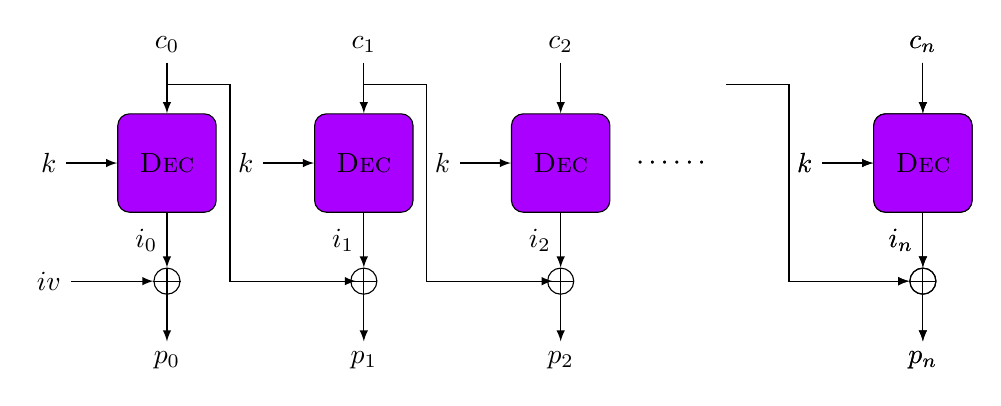
\begin{tikzpicture}
\tikzstyle{perm} = [minimum size=1.25cm,rounded
            corners=1ex,fill=primary,draw];


    \foreach \x in {0, 1, 2} {
        \node (f\x) at ($\x*(2.5cm,0)$) [perm] {{\sc Dec}};
        \node (c\x) [below of=f\x, node distance=2.5cm] {$p_\x$};
        \node (k\x) [left of=f\x, node distance=1.5cm] {$k$};
        \node (p\x) [below of=f\x, node distance=1.5cm, circle, draw] {};
        \node (m\x) [above of=f\x, node distance=1.5cm] {$c_\x$};
        \draw[-] (p\x.north) -- (p\x.south);
        \draw[-] (p\x.east) -- (p\x.west);
        \draw[-latex] (m\x) -- (f\x);
        \draw[-latex] (f\x) -- node[left] {$i_\x$} (p\x);
        \draw[-latex] (k\x) -- (f\x);
        \draw[-latex] (p\x) -- (c\x);
    }

    \node (iv) [left of=p0, node distance=1.5cm] {$iv$};
    \draw[-latex] (iv) -- (p0);

    \foreach \x in {0, 1} {
        \draw[-latex] ($(m\x) - (0,0.5cm)$) -| +(0.8cm,-2.5cm) -- ($(p\x) + (2.4cm,0)$);

    \begin{scope}
        \node at (6.4,0) {$\cdots\cdots$};
    \end{scope}

    \begin{scope}
        \node (f) at (9.6cm,0) [perm] {{\sc Dec}};
        \node (c) [below of=f, node distance=2.5cm] {$p_n$};
        \node (k) [left of=f, node distance=1.5cm] {$k$};
        \node (p) [below of=f, node distance=1.5cm, circle, draw] {};
        \node (m) [above of=f, node distance=1.5cm] {$c_n$};
        \draw[-] (p.north) -- (p.south);
        \draw[-] (p.east) -- (p.west);
        \draw[-latex] (m) -- (f);
        \draw[-latex] (f) -- node[left] {$i_n$} (p);
        \draw[-latex] (k) -- (f);
        \draw[-latex] (p) -- (c);
        \draw[-] ($(m) - (2.5,0.5cm)$) -- ($(m) - (1.7,0.5cm)$);
        \draw[-latex] ($(m) - (1.7,0.5cm)$) |- + (0cm,-2.5cm) -- (p);
    \end{scope}
    }

\end{tikzpicture}

\end{document}
